\documentclass[a4paper]{article}

%% Language and font encodings
\usepackage[spanish]{babel}
\usepackage[utf8x]{inputenc}
\usepackage[T1]{fontenc}

%% Sets page size and margins
\usepackage[a4paper,top=3cm,bottom=2cm,left=3cm,right=3cm,marginparwidth=2cm]{geometry}

%% Useful packages
\usepackage{amsmath}
\usepackage{graphicx}
\usepackage{float}
\usepackage[colorinlistoftodos]{todonotes}
\usepackage[colorlinks=true, allcolors=blue]{hyperref}

\title{Extendiendo DDColor: Análisis e 
investigación de las limitaciones del modelo.}
\author{José Carlos Mora López, Alejandro Parody Quirós, Guillermo Rodríguez Narbona}

\begin{document}
\maketitle

\begin{abstract}
 \noindent El resumen debe tener como máximo 250 palabras y ser un único párrafo. El resumen debe describir lo más fielmente posible el trabajo realizado (no el propuesto inicialmente, que podría ser distinto). 
 En esta plantilla se presentan las indicaciones para realizar el trabajo de PID, al mismo tiempo que la estructura que debe tener la documentación a presentar. 

\hspace{1cm}

\noindent \textbf{Palabras clave:} 
%(hasta cinco palabras que clasifiquen el trabajo) 
PID, colorización, imagen digital, red neuronal, limitaciones.
\end{abstract}


\section{Introducción}

En este trabajo, se realizó un análisis y extensión del proyecto DDColor \cite{DDColor}, el cual implementa un proceso de colorización de imágenes mediante una red neuronal.

Principalmente, este trabajo se centra en dos aspectos:

\begin{itemize}
  \item{Extensión de la red neuronal DDColor para su uso en imágenes no fotorrealistas mediante reentrenamiento.}
  \item{Estudio de las carencias del modelo a la hora de aplicar color a objetos translúcidos.}
\end{itemize}

Para ello, fue necesario realizar un análisis en profundidad de la arquitectura del sistema, así como de los mecanismos empleados.

\section{Planteamiento teórico}

El problema que busca resolver DDColor es el de la colorización de imágenes en escala de grises, el cual ha visto múltiples soluciones tanto manuales como en forma de algoritmos de procesamiento de imágenes digitales.

El novedoso método del proyecto DDColor consiste en una red neuronal que emplea una arquitectura \textit{encoder-decoder} \cite{IBMEncoderDecoder}.

Para la colorización, esta red emplea el modelo de color \textit{CIELAB}. De esta manera:
\begin{itemize}
  \item{La imagen original (en escala de grises) es tratada como el canal \textit{L} en dicho modelo de color (correspondiente a la luminancia).}
  \item{La función de la red es hallar los canales \textit{A} y \textit{B} (correspondientes a la crominancia).}
\end{itemize}

La red DDColor realiza los siguientes procesos:

\begin{enumerate}
  \item{Extracción de información semántica de los contenidos de la imagen (\textbf{encoder}).}
  \item{Construcción de un mapa de características de la imagen (\textbf{pixel decoder}).}
  \item{Construcción de una serie de \textit{colour queries} indicando cómo colorizar la imagen (\textbf{colour decoder}).}
  \item{Combinación de los resultados de los procesos anteriormente mencionados para aplicar color a la imagen (\textbf{fusion module}).}
\end{enumerate}

A continuación, se detallarán ambas partes de la arquitectura \textit{encoder-decoder}.

\subsection{Encoder}

La función del \textit{encoder} es convertir los datos de entrada a una representación vectorial. En el caso de la red DDColor, consiste en un modelo preentrenado, en este caso especializado en la clasificación de imágenes, encargado de la extracción de características semánticas de la imagen fuente.

\subsubsection{ConvNeXT}

El \textit{encoder} del proyecto DDColor es el modelo ConvNeXT \cite{ConvNeXT}, una red convolucional capaz de extraer una serie de mapas de características a distintas resoluciones (fracciones de la resolución original) que conforman una representación jerárquica de los contenidos de la imagen.

Dicho modelo surge como alternativa a los Vision Transformers (ViT) \cite{ViT}, introducidos como una aplicación de las arquitecturas basadas en \textit{transformers} (empleadas habitualmente en tareas de procesamiento de lenguaje natural) a la clasificación de imágenes, aplicación en la que tradicionalmente se habían empleado redes convolucionales.

Así, ConvNeXT introduce ideas originalmente presentadas en los Vision Transformers en una red puramente convolucional, combinando la mayor precisión ofrecida por éstos con la mayor eficiencia y sencillez de una red convolucional tradicional.

La arquitectura de ConvNeXT es la siguiente:

\begin{enumerate}
  \item{Capa de convolución con un kernel de tamaño 4x4 (\textit{patchify}).}
  \item{Cuatro ``stages'', cada uno con un número configurable de bloques con la misma estructura:}
  \begin{enumerate}
    \item{Capa de convolución \textit{depthwise} (se aplica la misma convolución a cada canal de la imagen por separado) con kernel de tamaño 7x7.}
    \item{Capa de normalización \textit{LayerNorm}.}
    \item{Capa de convolución con kernel de tamaño 1x1.}
    \item{Función de activación GELU (\textit{Gaussian Error Linear Unit}, similar a ReLU).}
    \item{Capa de convolución con kernel de tamaño 1x1.}
  \end{enumerate}
\end{enumerate}

De todo este proceso, es importante la inclusión de una capa de \textit{patchify}, la cual es una de las ideas introducidas en los Vision Transformers.

Esta capa se sitúa al inicio de la red, en lo que se denomina la \textit{stem cell} (encargada de procesar las imágenes al inicio para después ser tratadas por el resto de la red).

Su función es transformar la imagen en una serie de \textit{patches} (en el caso de esta red, mediante una convolución de 4x4). De esta manera, la secuencia de \textit{patches} generados en base a la imagen se emplearía como secuencia de entrada en un Vision Transformers (al estar las arquitecturas basadas en transformers especializadas en el procesamiento de secuencias).

Dicha capa se aplicó en ConvNeXT al comprobarse experimentalmente que mejoraba la precisión del modelo en comparación con las \textit{stem cells} empleadas en redes convolucionales convencionales.

Dependiendo del número de bloques y de canales en cada ``stage'', se distinguen múltiples variantes:

\begin{itemize}
  \item{ConvNeXT-T}
  \item{ConvNeXT-S}
  \item{ConvNeXT-B}
  \item{ConvNeXT-L}
  \item{ConvNeXT-XL}
\end{itemize}

En DDColor se utilizan las variantes ConvNeXT-T y ConvNeXT-L.

\subsection{Decoder}

El propósito del \textit{decoder} es convertir la salida vectorial del \textit{encoder} a una representación del mismo tipo que la inicial (en el caso de \textit{DDColor}, una imagen).

La arquitectura de DDColor comprende dos \textit{decoders} que trabajan simultáneamente (llamados \textit{pixel decoder} y \textit{colour decoder}).

\subsubsection{Pixel decoder}

Este decodificador emplea capas \textit{PixelShuffle} \cite{PixelShuffle} para reescalar los mapas de características producidos por el \textit{encoder} de vuelta a la resolución de la imagen fuente.

Cada capa \textit{PixelShuffle} contiene una secuencia de \textit{L} capas convolucionales, con la siguiente forma:

\begin{enumerate}
  \item{\textit{L-1} operaciones de convolución entre un kernel (matriz de pesos que se ajustan en el proceso de aprendizaje) y el resultado de la anterior capa (o la imagen fuente, en el caso de la primera capa).}
  \item{\textit{Operación de convolución con shuffle}: Tras la convolución, se aplica un operador que que reordena los elementos de la imagen, alterando sus dimensiones.}
\end{enumerate}

\subsubsection{Colour decoder}

Este decodificador emplea una arquitectura basada en la arquitectura de un transformer, es decir, empleando mecanismos de atención, para refinar \textit{colour queries}.

Dichas \textit{colour queries} son embeddings que indican el color de las distintas características de la imagen.

Para ello, se crean una serie de CDBs (\textit{Colour Decoder Blocks}), uno para cada mapa de características generado en el \textit{encoder}, los cuales procesan las \textit{colour queries} secuencialmente.

Cada CDB produce una salida (una \textit{colour query} refinada) en base a dos entradas:

\begin{itemize}
  \item{Mapa de características generado por el encoder.}
  \item{\textit{Colour query} a refinar.}
\end{itemize}

La \textit{colour query} inicial (la empleada como entrada del primer CDB de la secuencia) está inicializada al embedding nulo. El resto de CDBs emplean la \textit{colour query} refinada por el anterior CDB.

Antes de proceder con las operaciones realizadas dentro de cada CDB, se explicarán brevemente los mecanismos de atención empleados.

\paragraph{Mecanismos de atención}

Tienen tres características principales \cite{IBMAttention}:

\begin{enumerate}
  \item{Leen \textbf{secuencias de datos} y las transforman en \textit{embeddings} vectoriales.}
  \item{Asignan \textbf{pesos de atención} a los distintos elementos de la secuencia, determinando así su importancia.}
  \item{Implementan algún proceso para \textbf{influir en las predicciones del modelo} mediante los pesos de atención.}
\end{enumerate}

En los mecanismos de atención, para cada elemento de la secuencia, se distinguen tres conceptos fundamentales:

\begin{itemize}
  \item{\textbf{Query}: Vector que representa la información buscada por el elemento.}
  \item{\textbf{Key}: Vector que representa la información contenida por el elemento.}
  \item{\textbf{Value}: Vector que contiene la información del elemento, ponderada empleando los pesos de atención.}
\end{itemize}

La fórmula general de un mecanismo de atención es la siguiente \cite{Attention}:

\centerline{$Attention(Q, K, V) = softmax(\frac{QK^T}{\sqrt{d_k}})V$}

Donde:

\begin{itemize}
  \item{$d_k$ es la dimensión de las \textit{queries} y \textit{keys}.}
  \item{$softmax$ se refiere a la función de activación del mismo nombre, definida en \cite{Softmax}.}
\end{itemize}

En el contexto de DDColor, se emplean dos tipos de atención:

\begin{itemize}
  \item{\textbf{Atención cruzada}: Las \textit{queries} y las \textit{keys} provienen de fuentes distintas.}
  \item{\textbf{Autoatención}: Las \textit{queries} y las \textit{keys} proceden de la misma fuente.}
\end{itemize}

Las operaciones realizadas en cada CDB son las siguientes:

\begin{enumerate}
  \item{\textbf{Capa de atención cruzada} empleando el mapa de características como \textit{key} y \textit{value} y con la colour query como \textit{query}.}
  \item{\textbf{Capa de autoatención} empleando el resultado de la anterior como \textit{query}, \textit{key} y \textit{value}.}
  \item{\textbf{Red feed-forward} empleando el resultado de la anterior como entrada. Se trata de una red neuronal convencional, empleando la siguiente arquitectura:
    \begin{enumerate}
      \item{Capa lineal.}
      \item{Capa de \textit{drop-out} (cambia a 0 determinados valores del vector de entrada aleatoriamente según un valor probabilidad ajustable).}
      \item{Capa lineal.}
      \item{Capa de normalización.}
      \item{Función de activación ReLU.}
    \end{enumerate}
  }
\end{enumerate}

Entre cada par de capas, se aplica una capa de normalización. Además, en cada capa de normalización se suma el resultado de la anterior capa de normalización (funcionando así además como capas residuales).

\subsection{Fusión}

Tras el \textit{encoder} y el \textit{decoder}, la red DDColor contiene el denominado \textit{fusion module}, el cual realiza las siguientes operaciones:

\begin{enumerate}
  \item{Mediante un producto escalar, combinación del \textit{embedding} producido por el \textit{Pixel decoder} y el producido por el \textit{Colour decoder}.}
  \item{Aplicación de una operación de convolución con kernel de tamaño 1x1 para obtener los canales \textit{A} y \textit{B}.}
  \item{Concatenación de la imagen original en escala de grises (canal \textit{L}) y la imagen resultante de los dos pasos anteriores (canales \textit{A} y \textit{B}) para formar la imagen final.}
\end{enumerate}

\subsection{Métricas}
La forma en la que se analizan los resultados obtenidos por el modelo es mediante métricas de evaluación y comparación de imágenes.
Este aspecto resulta fundamental para el correcto estudio. Nos permite determinar automáticamente si las imágenes han sido peor o mejor colorizadas, y que conclusiones sacar de esos datos objetivos. 

Se trata de un dominio que creemos complicado. En el artículo original apenas se le dedica un pequeño párrafo, pues se da por supuesto el conocimiento de las distintas opciones que hay para realizar dicha evaluación. Nosotros creemos en el gran interés académico que tiene esta información, y también creemos que necesita de un análisis profundo para conocer las métricas que debemos usar. Nos planteamos también la pregunta: siendo que cambiamos de dominio con respecto al original (no-fotorrealista), ¿debemos plantearnos seleccionar distintas métricas de las que ya se han ofrecido?

Cabe mencionar que normalmente no basta con una sola métrica para analizar los resultados de un modelo, sino que se usa la combinación de varias para comprobar como funciona en distintos aspectos y tener un mejor análisis de los resultados.

En este apartado se discutirán las métricas ya utilizadas en el artículo original, y otras nuevas posibles alternativas que encajen mejor para evaluar nuestro modelo concreto. Las separaremos en dos bloques, aquellas que hemos descartado, y las dos que hemos seleccionado, que serán explicadas con más detalle.
\bigskip

\textbf{En definitiva, discutiremos FID, $\Delta CF$, PSNR (originales), $\Delta E$ y SSIM (nuevas)}

\subsubsection{Métricas descartadas}
Se presentan en esta sección aquellas métricas que han sido analizadas, pero descartadas por algún motivo, que será explicado en cada una. No se entrará en el detalle del funcionamiento, pretendiendo poder profundizar plenamente en las que si usaremos.

\paragraph{ • Fréchet Inception Distance: FID \cite{FID}}

El FID constituye la métrica principal en la que se basa el estudio original y representa uno de los indicadores más empleados en evaluación de imágenes generadas por sistemas de inteligencia artificial. Es crucial destacar que FID compara conjuntos amplios de imágenes contra otros conjuntos de magnitud similar; por tanto, su aplicabilidad depende de disponer de conjuntos de datos suficientemente grandes para garantizar resultados confiables.

Mide la distancia entre la distribución de características de imágenes generadas contra imágenes reales. Usa una red neuronal preentrenada (InceptionV3) para extraer características de alto nivel. Se suele utilizar para evaluación de imágenes generadas por IA.

A grandes rasgos, primeramente FID extrae  las características del conjunto de imágenes con la red neuronal. Luego sobre esas características, o features se calculan dos estadísticos clave para cada conjunto: la media de las características visuales detectadas y la matriz de covarianza. Finalmente, se mide la diferencia entre las estadísticas de ambos conjuntos.

\begin{table}[h]
	\centering
	\begin{tabular}{|p{0.45\textwidth}|p{0.45\textwidth}|}
		\hline
		\textbf{Ventajas} & \textbf{Desventajas} 
		\\ \hline
		- Correlaciona bien con percepción humana & - Depende del modelo de InceptionV3 (entrenado en fotografías naturales) \\
		- No depende de correspondencias pixel a pixel & - Puede sesgar evaluaciones en dominios no fotorrealistas \\
		 & - No evalúa precisión semántica de colores \\ 
		 & - Computacionalmente lenta \\ 
		 & - Compleja en su entendimiento y uso \\
		 & - Requiere de largos datasets \\ \hline
	\end{tabular}
\end{table}

\textbf{Razón de descarte:} Si bien FID promete un buen desempeño (por algo resulta la primera fuente de confianza del paper DDColor \cite{DDColor}) resulta ser demasiado compleja, no solo en su arquitectura que utiliza redes neurales externas, sino además en su uso, comparando dos grandes datasets, y los problemas que pueden derivar, véase, que no sea suficientemente grande para un buen rendimiento. Puesto que uno de los objetivos de este trabajo es el profundizamiento sobre procesos digitales, nos centraremos en otras métricas que funcionen a nivel local y que no dependan de IA. 

\paragraph{ • Peak Signal-to-Noise Ratio: PSNR \cite{PSNR}}

PSNR constituye una métrica clásica de similitud basada en comparación directa de valores RGB píxel a píxel. También fue utilizada en el paper DDColor \cite{DDColor}. Penaliza cualquier discrepancia numérica entre los píxeles de la imagen generada e imagen real, sin considerar que diferencias imperceptibles al ojo humano pueden generar variaciones significativas en el valor de PSNR.

Cabe mencionar que ya se decía en el artículo original que esta métrica no es la más indicada para reflejar trabajos de colorizacion. \cite{DDColor}, aunque igual se añade al conjunto de métricas para ampliar el análisis.

\begin{table}[h]
	\centering
	\begin{tabular}{|p{0.45\textwidth}|p{0.45\textwidth}|}
		\hline
		\textbf{Ventajas} & \textbf{Desventajas} 
		\\ \hline
		- Interpretación intuitiva de los resultados. & - Limitaciones en tareas específicas de colorización. \\
		- Alta eficiencia computacional. & - Sensibilidad extrema a desplazamientos espaciales (un pequeño movimiento de píxeles reduce drásticamente el PSNR). \\
		& - No refleja la fidelidad visual humana, centrándose únicamente en el error cuadrático promedio. \\ \hline
	\end{tabular}
\end{table}

\textbf{Razón de descarte:} Si bien PNSR trabaja mucho más rápido que FID, es más versátil, menos compleja y fácil de utilzar, no es ideal para colorización de imágenes. Creemos que existen otras alternativas que nos puedan dar información más valiosa sobre colorización, sin penalizar tanto las pequeñas discrepancias. 

\paragraph{ • Índice de Similitud Estructural: SSIM \cite{SSIM}}

SSIM es una métrica que no aparece en el paper original, pero que en algún momento consideramos añadir. A diferencia de PSNR, no realiza comparaciones exclusivamente a nivel de píxeles aislados, sino que analiza regiones locales de la imagen (ventanas normalmente de 11x11 pixeles) evaluando tres componentes: luminiscencia, contraste y estructura. El resultado final es un promedio ponderado de las similitudes locales. Debe considerarse que dos imágenes con estructura idéntica pero colores completamente distintos pueden obtener valores SSIM elevados.

\begin{table}[h]
	\centering
	\begin{tabular}{|p{0.45\textwidth}|p{0.45\textwidth}|}
		\hline
		\textbf{Ventajas} & \textbf{Desventajas} 
		\\ \hline
		- Métrica estable y ampliamente utilizada en evaluación de imágenes & - No realiza análisis semántico del acierto en colorización \\
		- Alta eficiencia computacional. & - Principalmente captura estructura, no es importante para colorización \\
		- Rápida y facil de usar & - Como la estructura es idéntica, SSIM tiende a valores muy altos en casi todos los casos \\ \hline
	\end{tabular}
\end{table}

\textbf{Razón de descarte:} Al igual que ocurre con PSNR, SSIM nos ofrece una métrica rápida y versátil, idependiente de modelos de redes neuronales; pero que no encaja con el dominio de colorización de imágenes.


\subsubsection{Métricas utilizadas}

Las métricas seleccionadas finalmente han sido $\Delta CF$ y $\Delta E$, debido a su enfoque directo en la cuantificación de diferencias de color, que constituye el objetivo principal del análisis. Frente a alternativas como FID, que implica el uso de modelos de IA preentrenados y añade una complejidad computacional innecesaria para este contexto, o métricas tradicionales como SSIM y PSNR, más orientadas a evaluar similitud estructural o fidelidad de señal, pero con escasa sensibilidad específica al color, $\Delta CF$ y  $\Delta E$ ofrecen una evaluación más precisa y relevante. De este modo, se priorizan métricas interpretables, específicas y alineadas con la naturaleza del problema abordado.
Veamoslas con más detalle.

\paragraph{ • Colorfulness Score: CF \cite{CF}}

La métrica $\Delta CF$ se fundamenta en la comparación del \textit{Colorfulness} (CF) entre dos imágenes. El término CF hace referencia a la percepción subjetiva de la viveza o intensidad cromática de una imagen, es decir, cómo de “colorida” resulta visualmente. Esta medida fue diseñada específicamente para capturar propiedades relacionadas con la distribución y variabilidad del color, a diferencia de otras métricas que priorizan aspectos estructurales o de luminancia.

El objetivo de $\Delta CF$ es cuantificar la variación global de color entre dos imágenes mediante la diferencia entre sus respectivos valores de CF. De este modo, se obtiene una medida directa del cambio en la percepción cromática.

\medskip
\textbf{Espacio de color y canales utilizados}

El cálculo de CF se realiza partiendo del espacio de color RGB, donde cada píxel está representado por tres canales: rojo ($R$), verde ($G$) y azul ($B$). Sin embargo, la métrica no opera directamente sobre estos tres canales de forma independiente, sino que transforma la información en dos componentes cromáticas diseñadas para aproximar la percepción humana del color.

Estas componentes son:

\begin{itemize}
	\item Diferencia rojo-verde:
	\begin{equation}
		rg = R - G
	\end{equation}
	
	\item Diferencia amarillo-azul:
	\begin{equation}
		yb = \frac{1}{2}(R + G) - B
	\end{equation}
\end{itemize}

Estas transformaciones combinan los tres canales RGB en dos ejes cromáticos principales. Por tanto, aunque el cálculo de CF utiliza información proveniente de los tres canales originales, no se evalúan de manera independiente, sino a través de estas dos componentes que capturan relaciones perceptuales entre ellos.

\medskip
\textbf{Cálculo del Colorfulness (CF)}

El algoritmo para calcular CF sigue los siguientes pasos:

\begin{enumerate}
	\item Para cada píxel de la imagen, se calculan las componentes $rg$ y $yb$ a partir de los valores de $R$, $G$ y $B$.
	
	\item Se obtienen la media y la desviación estándar de ambas componentes en toda la imagen:
	\begin{equation}
		\mu_{rg}, \quad \sigma_{rg}
	\end{equation}
	\begin{equation}
		\mu_{yb}, \quad \sigma_{yb}
	\end{equation}
	
	\item Se combinan estos valores para obtener la medida de Colorfulness:
	\begin{equation}
		CF = \sqrt{\sigma_{rg}^2 + \sigma_{yb}^2} + 0.3 \cdot \sqrt{\mu_{rg}^2 + \mu_{yb}^2}
	\end{equation}
\end{enumerate}

El primer término de la ecuación mide la dispersión de los colores (variabilidad), mientras que el segundo introduce un ajuste basado en el sesgo medio de las componentes cromáticas.

\medskip
\textbf{Cálculo de $\Delta CF$}

Una vez obtenido el valor de CF para cada una de las dos imágenes a comparar, la métrica $\Delta CF$ se define como:

\begin{equation}
	\Delta CF = | CF_1 - CF_2 |
\end{equation}

donde $CF_1$ y $CF_2$ representan los valores de Colorfulness de cada imagen.

Esta diferencia permite evaluar de forma directa el cambio en la viveza cromática global entre ambas imágenes. Un valor elevado de $\Delta CF$ indica una diferencia notable en la intensidad o riqueza del color, mientras que valores cercanos a cero sugieren una apariencia cromática similar.

\paragraph{ • Color diference: $\Delta E$ \cite{DeltaE}}


La métrica $\Delta E$ se utiliza para cuantificar la diferencia perceptual entre dos colores. A diferencia de métricas basadas en RGB, $\Delta E$ se define en espacios de color perceptualmente uniformes, como CIELAB, donde las distancias euclidianas se corresponden mejor con las diferencias percibidas por el ojo humano.

En el contexto de comparación de imágenes, $\Delta E$ permite evaluar cuánto difieren dos imágenes en términos de color a nivel perceptual, siendo especialmente útil en aplicaciones donde la fidelidad cromática es crítica.


Existen varias formas de calcular Color Difference. Nosotros usaremos la métrica $\Delta E_{2000}$ representa el estado del arte en la cuantificación de diferencias perceptuales de color. A diferencia de formulaciones anteriores como $\Delta E_{76}$, que se basan en distancias euclídeas simples en el espacio CIELAB, $\Delta E_{2000}$ introduce una serie de correcciones no lineales diseñadas para ajustar la medida a la percepción real del ojo humano.

Estas mejoras tienen en cuenta que la sensibilidad visual no es uniforme en todo el espacio de color, y que las diferencias en luminosidad, croma y tono no contribuyen de la misma manera a la percepción global.

\medskip
\textbf{Espacio de color CIELAB}

Cada píxel se representa en el espacio CIELAB mediante tres componentes:

\begin{itemize}
	\item $L^*$: luminosidad
	\item $a^*$: componente verde-rojo
	\item $b^*$: componente azul-amarillo
\end{itemize}

Este espacio permite trabajar con magnitudes más alineadas con la percepción humana, siendo la base para el cálculo de $\Delta E$.

\medskip
\textbf{Descripción del algoritmo}

El cálculo de $\Delta E_{2000}$ entre dos píxeles $(L_1, a_1, b_1)$ y $(L_2, a_2, b_2)$ se realiza mediante los siguientes pasos:

\begin{enumerate}
	
	\item \textbf{Cálculo del croma}
	
	Se calcula el croma de cada color como:
	
	\begin{equation}
		C_i = \sqrt{a_i^2 + b_i^2}
	\end{equation}
	
	El croma representa la intensidad del color (saturación). Este paso permite separar la información de color en magnitudes más interpretables perceptualmente.
	
	\item \textbf{Ajuste del eje $a^*$}
	
	Se introduce un factor de corrección $G$ que modifica el canal $a^*$:
	
	\begin{equation}
		a'_i = (1 + G)a_i
	\end{equation}
	
	Este ajuste corrige desviaciones perceptuales, especialmente en colores cercanos al gris, donde el modelo CIELAB presenta menor precisión.
	
	\item \textbf{Nuevo croma y cálculo del tono}
	
	Con los valores ajustados, se recalcula el croma:
	
	\begin{equation}
		C'_i = \sqrt{a'^2_i + b_i^2}
	\end{equation}
	
	y el tono:
	
	\begin{equation}
		h'_i = \arctan\left(\frac{b_i}{a'_i}\right)
	\end{equation}
	
	El tono representa el tipo de color (rojo, azul, etc.), y se expresa como un ángulo.
	
	\item \textbf{Cálculo de diferencias}
	
	Se obtienen las diferencias en cada componente:
	
	\begin{equation}
		\Delta L', \quad \Delta C', \quad \Delta H'
	\end{equation}
	
	La diferencia de tono $\Delta H'$ se calcula de forma especial para evitar discontinuidades angulares, asegurando continuidad perceptual.
	
	\item \textbf{Factores de ponderación}
	
	Se introducen factores de escala:
	
	\begin{equation}
		S_L, \quad S_C, \quad S_H
	\end{equation}
	
	Estos factores ajustan la importancia relativa de cada componente (luminosidad, croma y tono), reflejando que el ojo humano no percibe todas las variaciones con la misma sensibilidad.
	
	\item \textbf{Término de interacción}
	
	Se incorpora un término de rotación $R_T$, que modela la interacción entre croma y tono:
	
	\begin{equation}
		R_T
	\end{equation}
	
	Este término corrige regiones específicas del espacio de color (especialmente tonos azulados) donde las diferencias perceptuales no son lineales.
	
	\item \textbf{Cálculo final}
	
	La diferencia de color se obtiene como:
	
	\begin{equation}
		\Delta E_{2000} =
		\sqrt{
			\left(\frac{\Delta L'}{S_L}\right)^2 +
			\left(\frac{\Delta C'}{S_C}\right)^2 +
			\left(\frac{\Delta H'}{S_H}\right)^2 +
			R_T \cdot \frac{\Delta C'}{S_C} \cdot \frac{\Delta H'}{S_H}
		}
	\end{equation}
	
\end{enumerate}

\medskip
\textbf{Aplicación a imágenes}

Para comparar dos imágenes, el proceso se realiza píxel a píxel:

\begin{enumerate}
	\item Convertir ambas imágenes a CIELAB.
	\item Calcular $\Delta E_{2000}$ para cada par de píxeles correspondientes.
	\item Obtener una medida global mediante la media:
	\begin{equation}
		\Delta E = \frac{1}{N} \sum_{i=1}^{N} \Delta E_{2000}(i)
	\end{equation}
\end{enumerate}

\medskip
\textbf{Interpretación}

Valores bajos de $\Delta E_{2000}$ indican diferencias apenas perceptibles, mientras que valores altos corresponden a cambios visibles en el color. Esta métrica proporciona una medida robusta y alineada con la percepción humana, lo que justifica su uso como estándar en aplicaciones de análisis de color.

\section{Implementación}

Para este proyecto, se realizó un \textit{fork} del repositorio de GitHub en el que reside la implementación de la red DDColor:

\begin{itemize}
  \item{Repositorio original: \url{https://github.com/piddnad/DDColor}.}
  \item{\textit{Fork} realizado para el proyecto: \url{https://github.com/grnln/DDColor}.}
\end{itemize}

La red en cuestión fue implementada en \href{https://www.python.org/}{Python}, empleando principalmente las librerías \href{https://pytorch.org/}{PyTorch} (\textit{framework} para la implementación de redes neuronales) y \href{https://numpy.org/}{NumPy} (librería especializada en la implementación de operaciones matemáticas de forma vectorial).

Asimismo, se emplean otras librerías en el proyecto:

\begin{itemize}
  \item{\href{https://opencv.org/}{OpenCV}: Implementa múltiples operaciones de visión por ordenador.}
  \item{\href{https://pillow.readthedocs.io/en/stable/}{Pillow}: Implementa operaciones de lectura y procesamiento de imágenes.}
  \item{\href{https://tqdm.github.io/}{tqdm}: Implementa barras de progreso para aplicaciones de línea de comandos de forma sencilla.}
  \item{\href{https://huggingface.co/}{HuggingFace}: Librería implementada por la comunidad de inteligencia artificial homónima para cargar modelos almacenados en su servicio web.}
\end{itemize}

Por último, el proceso de entrenamiento de la red también requiere las siguientes dependencias:

\begin{itemize}
  \item{\href{https://pyyaml.org/}{PyYAML}: Implementa operaciones de gestión de ficheros en formato YAML en Python.}
  \item{\href{https://scikit-image.org/}{Scikit-image}: Implementa operaciones de procesamiento de imágenes.}
  \item{\href{https://scipy.org/}{SciPy}: Implementa algoritmos para computación científica.}
  \item{\href{https://www.tensorflow.org/tensorboard}{TensorBoard}: Implementa herramientas de visualización para la experimentación de machine learning (parte del proyecto TensorFlow).}
  \item{\href{https://wandb.ai/site/}{Weights \& Biases}: Implementa un \textit{framework} para gestionar modelos de inteligencia artificial.}
\end{itemize}

El código está principalmente contenido en tres directorios del repositorio:

\begin{itemize}
  \item{El directorio \texttt{ddcolor} contiene la implementación de la propia red DDColor.}
  \item{El directorio \texttt{basicsr} contiene \href{https://github.com/xpixelgroup/basicsr}{BasicSR}, un conjunto de herramientas para la restauración de imagen y vídeo que es empleado por DDColor como \textit{framework} de entrenamiento.}
  \item{El directorio \texttt{scripts} contiene una serie de pequeños scripts, empleados para realizar varias tareas.}
\end{itemize}

Adicionalmente, el directorio raíz del repositorio contiene un archivo \texttt{setup.py}, empleado para realizar la configuración inicial del proyecto.

\subsection{DDColor}

En el directorio \texttt{ddcolor} reside la implementación de la red DDcolor, contenida en dos archivos:

\begin{itemize}
  \item{\texttt{model.py}: Contiene la implementación del modelo en sí.}
  \item{\texttt{pipeline.py}: Contiene la implementación de la \textit{pipeline} empleada para colorizar imágenes mediante DDColor.}
\end{itemize}

A continuación, se analizarán ambos módulos por separado.

\subsubsection{Modelo}

El modelo DDColor se implementa como tres módulos de Torch:

\begin{itemize}
  \item{\texttt{DDColor}: Implementa la arquitectura de la red a alto nivel, invocando a los demás módulos internamente cuando sea necesario.}
  \item{\texttt{ImageEncoder}: Implementa la sección del \textit{encoder}, invocando a la red ConvNeXT (preentrenada) internamente.}
  \item{\texttt{DuelDecoder}: Implementa la arquitectura de la sección del \textit{decoder} a alto nivel, invocando tanto a una versión customizada de PixelShuffle (\textit{pixel decoder}) como al módulo \texttt{MultiScaleColorDecoder} (\textit{colour decoder}) internamente.}
  \item{\texttt{MultiScaleColorDecoder}: Implementa la sección correspondiente al \textit{colour decoder}, implementando una arquitectura similar a un transformer.}
\end{itemize}

A continuación se explicará en mayor profundidad cómo funciona cada uno de ellos.

\paragraph{Módulo DDColor}

Este módulo permite configurar varios parámetros de la red mediante su constructor, entre los cuales se hallan:

\begin{itemize}
  \item{\textit{Encoder} a utilizar: Por defecto, \texttt{``convnext-l''} (ConvNeXT).}
  \item{\textit{Decoder} a utilizar: Por defecto, \texttt{MultiScaleColorDecoder}.}
  \item{Tamaño de entrada: Por defecto, 256x256 píxeles y 3 canales.}
  \item{Número de canales de salida: Por defecto, 3.}
  \item{Número de \textit{colour queries} a emplear para la colorización: Por defecto, 256.}
\end{itemize}

La mayoría de estos parámetros se emplean después como parámetros de entrada para los módulos instanciados internamente.

Este módulo define tanto el \textit{encoder} como el \textit{decoder} a utilizar (instanciándolos como módulos de Torch para su uso interno) y, además, instancia una capa de convolución custom (procedente de \texttt{BasicSR}) con un kernel de tamaño 1x1 para realizar la fusión.

Cuando este módulo es invocado, sencillamente invoca a la instancia del \texttt{ImageEncoder} construida, luego a la instancia del \texttt{DuelDecoder}, y posteriormente a la capa de refinación (convolución de 1x1) para la fusión.

\paragraph{Módulo ImageEncoder}

Este módulo actúa principalmente como un \textit{wrapper} en torno a ConvNeXT.

Permite configurar los siguientes parámetros:

\begin{itemize}
  \item{Nombre del \textit{encoder} a emplear: Por defecto se emplea \texttt{``convnext-l''}.}
  \item{\textit{Hooks} a añadir al \textit{decoder}.}
\end{itemize}

El módulo se limita a instanciar ConvNeXT con los parámetros adecuados.

En primer lugar, el nombre del \textit{encoder} actúa como un potencial punto de variabilidad del sistema, al teóricamente permitir conectar múltiples modelos diferentes a la red, mas la implementación lo restringe a solo dos posibles valores: \texttt{``convnext-t''} y \texttt{``convnext-l''}.

De esta manera, este parámetro solo determina las ``profundidades'' del modelo ConvNeXT a instanciar, es decir, el número de bloques que habrá en cada \textit{stage} del modelo ConvNeXT instanciado.

Posteriormente, los \textit{hooks} se ajustan mediante una lista de cadenas de texto, y no son realmente configurables por el usuario de DDColor, sino que el módulo \texttt{DDColor} los ajusta manualmente al construir la instancia.

En cuanto a su propósito, indican en qué puntos extraer el estado actual del mapa de características generado (lo cual es necesario para extraer los mapas de características a distintas resoluciones que se envían como \textit{shortcut connections} al \textit{colour decoder}).

Cuando este módulo es invocado, invoca a la instancia de ConvNeXT construida.

\paragraph{Módulo DuelDecoder}

Este módulo recibe como parámetro de entrada la lista de \textit{hooks} también introducida en el anterior módulo y actúa como un wrapper sobre los dos \textit{decoders} de la red:

\begin{itemize}
  \item{El \textit{pixel decoder}, implementado directamente en este módulo como una sucesión de capas PixelShuffle modificadas.}
  \item{El \textit{colour decoder}, implementado en el módulo \texttt{MultiScaleColorDecoder}.}
\end{itemize}

Además, permite ajustar, entre otros, los siguientes parámetros:

\begin{itemize}
  \item{Nombre del \textit{colour decoder} a emplear: Por defecto \texttt{``MultiScaleColorDecoder''}, el cual a su vez es el único valor tolerado por la propiedad.}
  \item{Número de \textit{queries} a refinar en el \textit{colour decoder}.}
\end{itemize}

La estructura empleada para el \textit{pixel decoder} consiste en una serie de instancias del módulo \texttt{UNetBlockWide} (definido en \texttt{BasicSR}), que a su vez está construido en torno a una versión personalizada de una capa PixelShuffle.

Se añade una instancia para cada \textit{hook} añadido al \textit{encoder}, comenzando por el último y exceptuando el primero, y, para el primer hook, una instancia directa de la capa PixelShuffle personalizada.

\paragraph{Módulo MultiScaleColorDecoder}

Este módulo se encarga de implementar el \textit{colour decoder}, empleando para ello una arquitectura similar a la de un transformer.

Tiene, entre otros, los siguientes parámetros configurables:

\begin{itemize}
  \item{Número de \textit{colour queries} a aprender y refinar (por defecto, 100).}
  \item{Númreo de capas a emplear (número de CDBs a emplear), por defecto 9.}
  \item{Dimensión intermedia de la \textit{feed-forward network}.}
\end{itemize}

Además, este módulo se encarga de inicializar los \textit{embeddings} a emplear para la decodificación.

Aparte de instanciar la arquitectura que se explicó en la sección correspondiente del planteamiento teórico, este módulo instancia también una capa de codificación posicional (\texttt{PositionEmbeddingSine}, definida en \texttt{BasicSR}), la cual se emplea para generar un \textit{embedding} posicional en base a la entrada de la red.

\subsubsection{Pipeline}

\subsection{BasicSR}

\subsection{Scripts}

\subsection{Contribución propia}

\section{Experimentación}

En este sección se verán los resultados realizados sobre la colorización de un total de 10 imágenes distintas, referidas al dominio no fotorrealista. Cada imagen ha sido coloreada usando, no solo nuestro modelo, sino tambien el modelo DDColor ''modelscope'' que es el que usan en el paper, asi como DDColor ``artistic``, un modelo que fue entrenado con datasets de arte (pero referido a pintura). 

\begin{figure}[H]
	\centering
	\includegraphics[width=\textwidth]{../assets/images/composicion2.jpg}
	\caption{Comparacion imagenes con distintos modelos}
	\label{fig:comparacion2}
\end{figure}
\begin{figure}[H]
	\centering
	\includegraphics[width=\textwidth]{../assets/images/composicion.jpg}
	\caption{Comparacion imagenes con distintos modelos}
	\label{fig:comparacion1}
\end{figure}

\section{Manual de usuario}

La aplicación \textit{DDColor Lab} es una herramienta de escritorio desarrollada en Python que permite colorizar imágenes en escala de grises mediante los modelos DDColor y comparar los resultados de forma visual y cuantitativa.

\subsection{Instalación del entorno}

Para ejecutar la aplicación es necesario tener instaladas las siguientes dependencias:

\begin{itemize}
	\item \texttt{Python}: Version superior o igual a 3.10
	\item \texttt{PyTorch}: Version superior o igual a 1.7
	\texttt{torchvision}: framework de redes neuronales.
	\item \texttt{opencv-python}: operaciones de visión por ordenador.
	\item \texttt{pillow}: lectura y procesamiento de imágenes.
	\item \texttt{scikit-image}: necesario para el cálculo de la métrica $\Delta E$.
	
\end{itemize}

\subsubsection{Creación del entorno}

El siguiente comando crea un entorno Conda aislado con Python:

\begin{verbatim}
conda create -n ddcolor python=3.9
conda activate ddcolor
\end{verbatim}

Como alternativa, puede crearse un entorno virtual independiente de Python:

\begin{verbatim}
python -m venv venv
source venv/bin/activate        # Linux / macOS
venv\Scripts\activate           # Windows
\end{verbatim}

\subsubsection{Dependencias}

Una vez activado el entorno, se instala PyTorch con soporte para CUDA 11.8. Si no se dispone de GPU compatible, puede omitirse el argumento \texttt{--index-url} y se instalará la versión de CPU:

\begin{verbatim}
pip install torch==2.2.0 torchvision==0.17.0 \
    --index-url https://download.pytorch.org/whl/cu118
\end{verbatim}

Las dependencias necesarias para ejecutar la inferencia se instalan con:

\begin{verbatim}
pip install -r requirements.txt
\end{verbatim}

\subsection{Descarga de modelos}

Previo a la ejecución del programa, deben descargarse los pesos de los tres modelos que se evalúan y colocarse dentro de una carpeta \texttt{./models/} en la raíz del proyecto. \textbf{IMPORTANTE: Los archivos descargados de tipo \texttt{.bin} deben renombrarse con extensión \texttt{.pth}. Deben respetarse exactamente los nombres \texttt{ddcolor\_comic.pth}, \texttt{ddcolor\_realistic.pth} y \texttt{ddcolor\_artistic.pth}.}

Los enlaces de descarga directa desde el navegador son:

\begin{itemize}
  \item \texttt{ddcolor\_comic.pth}: modelo fine-tuned sobre imágenes de cómic.\\
  \url{https://huggingface.co/Aleparqui/PID_proyect/blob/main/net_g_latest.pth}

  \item \texttt{ddcolor\_realistic.pth}: modelo oficial de ModelScope (realista).\\
  \url{https://huggingface.co/piddnad/ddcolor_modelscope/blob/main/pytorch_model.bin}

  \item \texttt{ddcolor\_artistic.pth}: modelo artístico de ModelScope.\\
  \url{https://huggingface.co/piddnad/ddcolor_artistic/blob/main/pytorch_model.bin}
\end{itemize}

\subsubsection{Ejemplo de descarga desde el navegador}

A continuación se ilustra el proceso con \texttt{ddcolor\_comic}. Repetir con cada modelo.

\paragraph{PASO 1:} Acceder al enlace del modelo, en este caso:\\
\url{https://huggingface.co/Aleparqui/PID_proyect/blob/main/net_g_latest.pth}

\paragraph{PASO 2:} Pulsar el botón \textit{Download} situado en la parte superior izquierda de la página (ver Figura~\ref{fig:captura_hf}).

\begin{figure}[H]
  \centering
  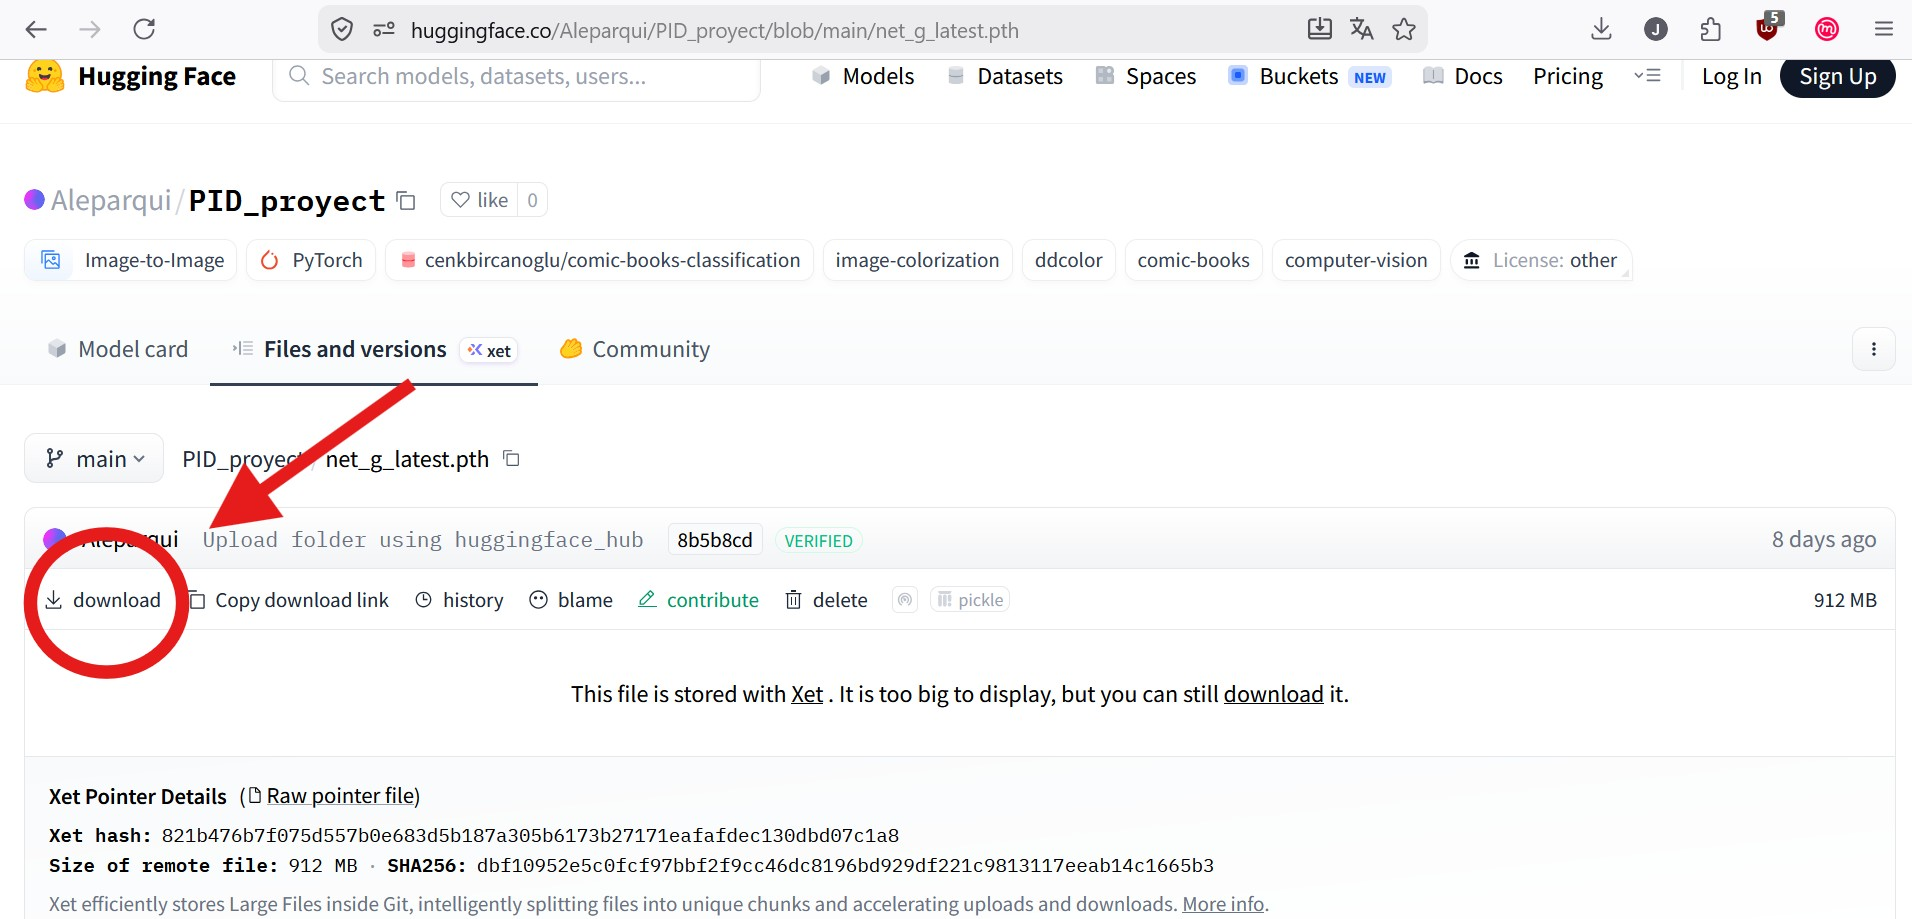
\includegraphics[width=\textwidth]{../assets/images/captura_hf.jpg}
  \caption{Captura de Hugging Face para descargar el modelo.}
  \label{fig:captura_hf}
\end{figure}

\paragraph{PASO 3:} Renombrar el archivo correctamente y colocarlo dentro de la carpeta \texttt{DDColor/models} (ver Figura~\ref{fig:captura_explorador}).

\begin{figure}[H]
  \centering
  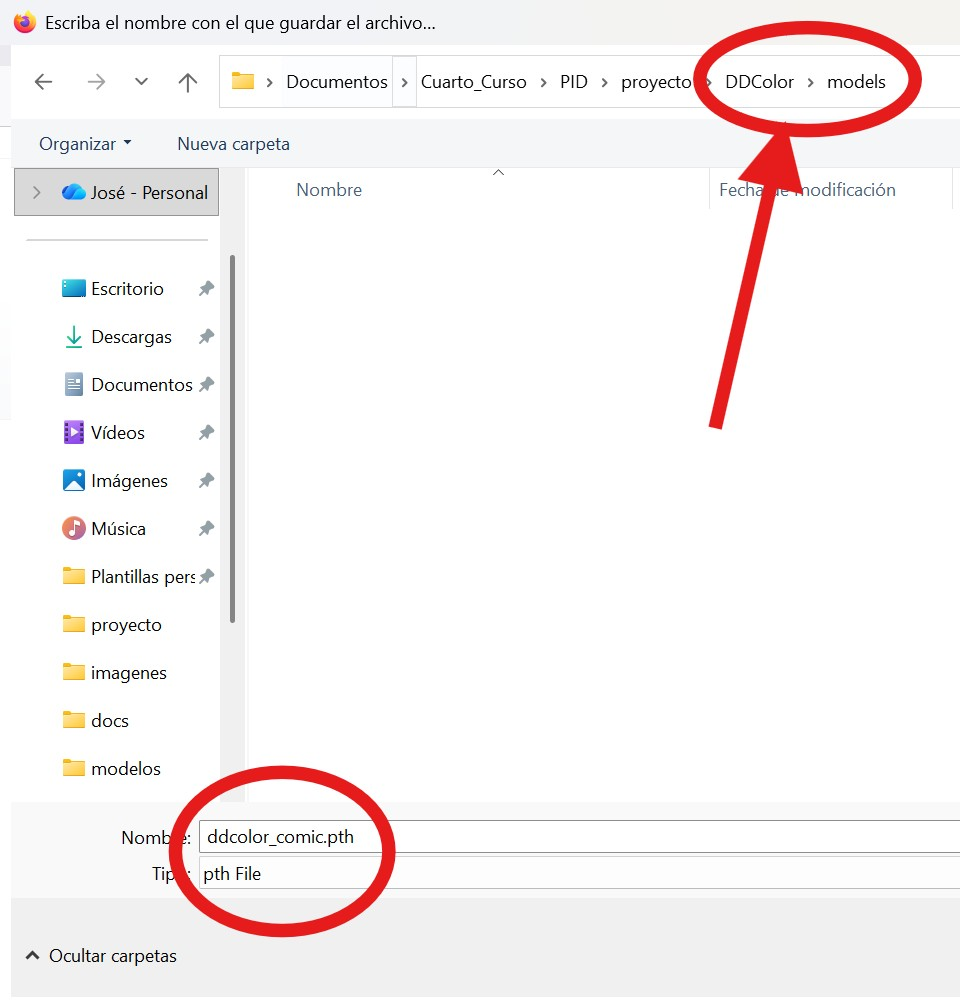
\includegraphics[width=0.5\textwidth]{../assets/images/captura_explorador.jpg}
  \caption{Captura del explorador de archivos con los pesos correctamente ubicados.}
  \label{fig:captura_explorador}
\end{figure}

\subsubsection{Descarga programática}

Como alternativa, los tres ficheros pueden descargarse automáticamente con \texttt{huggingface\_hub}:

\begin{verbatim}
pip install huggingface_hub

from huggingface_hub import hf_hub_download

# Modelo cómic (fine-tune propio)
hf_hub_download(repo_id="Aleparqui/PID_proyect",
                filename="net_g_latest.pth",
                local_dir="./models/")
# Renombrar a ddcolor_comic.pth

# Modelo realista
hf_hub_download(repo_id="piddnad/ddcolor_modelscope",
                filename="pytorch_model.bin",
                local_dir="./models/")
# Renombrar a ddcolor_realistic.pth

# Modelo artístico
hf_hub_download(repo_id="piddnad/ddcolor_artistic",
                filename="pytorch_model.bin",
                local_dir="./models/")
# Renombrar a ddcolor_artistic.pth
\end{verbatim}

Si alguno de los pesos no está disponible, la aplicación entra automáticamente en \textbf{modo DEMO} para ese modelo, aplicando una colorización sintética sin necesidad de ejecutar la red neuronal.

\subsection{Puesta en marcha}

Una vez cumplidos los requisitos y descargados los tres modelos, la aplicación se lanza ejecutando:

\begin{verbatim}
python ddcolor_desktop.py
\end{verbatim}

\textbf{IMPORTANTE:} Al iniciarse, la aplicación carga los modelos en segundo plano e indica su estado en la esquina superior derecha de la ventana. Esperar a que carguen y a que aparezca el mensaje \textit{Listo} en verde.

\subsection{Interfaz}

La ventana principal se divide en tres pestañas:

\begin{itemize}
  \item \textbf{Colorizar y comparar}: flujo principal de uso.
  \item \textbf{Métricas}: tabla comparativa con los resultados numéricos de la última colorización.
  \item \textbf{Guía}: documentación integrada sobre instalación, modelos y métricas.
\end{itemize}

\subsection{Flujo de uso}

\subsubsection{Cargar una imagen}

En el panel izquierdo, pulsar el botón \textit{Abrir imagen} o hacer clic sobre la miniatura. Se abrirá un explorador de archivos que admite los formatos \texttt{PNG}, \texttt{JPG}, \texttt{BMP}, \texttt{TIFF} y \texttt{WebP}. La imagen seleccionada se mostrará como miniatura y se usará automáticamente como \textit{ground truth} para el cálculo de métricas.

\subsubsection{Seleccionar un ground truth alternativo (opcional)}

Si se dispone de una versión coloreada de referencia distinta a la propia imagen de entrada, puede cargarse mediante el botón \textit{Abrir GT (opcional)}. Esto permite obtener métricas comparativas más significativas cuando se trabaja con imágenes originalmente en escala de grises.

\subsubsection{Seleccionar los modelos}

Las tres casillas de verificación del panel izquierdo permiten activar o desactivar individualmente cada modelo:

\begin{itemize}
  \item \textbf{Cómic FT} (azul): modelo fine-tuned sobre el dataset de cómics.
  \item \textbf{Realista HF} (morado): modelo oficial de DDColor orientado a fotografía.
  \item \textbf{Artístico HF} (naranja): modelo oficial de DDColor con estilo artístico.
\end{itemize}

\subsubsection{Ejecutar la colorización}

Pulsar el botón \textit{Ejecutar}. La barra de progreso indica que el proceso está en curso. Una vez finalizado, los resultados se muestran en el panel derecho: el modelo Cómic FT en la columna izquierda, y los modelos Realista y Artístico en pestañas intercambiables en la columna derecha.

\subsubsection{Consultar las métricas}

Navegar a la pestaña \textbf{Métricas} para ver la tabla comparativa. Para cada métrica, se marca en verde el modelo que obtiene el mejor resultado. Las métricas disponibles son:

\begin{itemize}
  \item $\Delta CF$: diferencia en viveza cromática respecto al ground truth. Valores cercanos a 0 indican que la paleta de color es similar a la referencia.
  \item $\Delta E_{2000}$: error colorimétrico perceptual medio píxel a píxel en el espacio CIELAB. Un valor menor implica mayor fidelidad de color.
\end{itemize}

\subsubsection{Guardar los resultados}

Pulsar el botón \textit{Guardar resultados} para exportar las imágenes colorizadas a una carpeta de destino. Se generan hasta tres archivos \texttt{PNG}:

\begin{itemize}
  \item \texttt{result\_comic\_ft.png}
  \item \texttt{result\_realistic\_hf.png}
  \item \texttt{result\_artistic\_hf.png}
\end{itemize}

Solo se exportan los modelos que estaban activos y produjeron un resultado.

\subsection{Publicación de los pesos en Hugging Face}

Con el objetivo de facilitar la reproducibilidad del trabajo y permitir que cualquier usuario pueda utilizar el modelo fine-tuned sin necesidad de reentrenarlo, los pesos resultantes del entrenamiento se han publicado en Hugging Face, una plataforma ampliamente utilizada en la comunidad de inteligencia artificial para alojar y compartir modelos, datasets y aplicaciones de forma pública y gratuita.

Hugging Face organiza los modelos en repositorios con control de versiones basado en Git, de forma análoga a GitHub pero orientada específicamente a ficheros de gran tamaño como pesos de redes neuronales. Cada repositorio incluye una \textit{Model Card}, un documento en formato Markdown que describe el modelo, su entrenamiento y cómo utilizarlo.

El repositorio del proyecto se encuentra en:

\begin{center}
  \url{https://huggingface.co/Aleparqui/PID_proyect}
\end{center}

\subsubsection{Contenido del repositorio}

El repositorio está registrado como modelo de tipo \textit{Image-to-Image} con las etiquetas \texttt{image-colorization}, \texttt{ddcolor} y \texttt{comic-books}, lo que lo hace indexable y localizable dentro de la plataforma. Contiene dos elementos principales:

\begin{itemize}
  \item \textbf{Fichero de pesos} \texttt{net\_g\_latest.pth}: generado automáticamente por BasicSR al finalizar el entrenamiento. El nombre \texttt{latest} indica que corresponde al estado del generador en la última iteración completada. Este fichero es el que debe descargarse para usar el modelo en la aplicación o en cualquier script de inferencia.

  \item \textbf{Model Card}: documento en formato Markdown redactado desde la interfaz web de Hugging Face. Recoge la descripción del modelo, el modelo base del que parte (\texttt{piddnad/ddcolor\_modelscope}), el dataset de entrenamiento empleado, los hiperparámetros principales y ejemplos de código para realizar inferencias.
\end{itemize}

\subsubsection{Proceso de subida}

La subida de los pesos se realizó mediante la herramienta de línea de comandos \texttt{huggingface\_hub}, siguiendo estos pasos:

\begin{enumerate}
  \item \textbf{Creación de la cuenta y el repositorio} en \url{https://huggingface.co}. Al crear el repositorio se seleccionó el tipo \textit{Model} y se activó la visibilidad pública para que cualquier usuario pueda acceder a los pesos sin necesidad de autenticación.

  \item \textbf{Instalación de la herramienta} en el entorno local:
  \begin{verbatim}
  pip install huggingface_hub
  \end{verbatim}

  \item \textbf{Autenticación local} mediante un token de acceso personal, generado desde los ajustes de la cuenta en la web de Hugging Face (\textit{Settings} $\rightarrow$ \textit{Access Tokens}):
  \begin{verbatim}
  huggingface-cli login
  \end{verbatim}
  El comando solicita el token por consola y lo almacena localmente para las operaciones posteriores.

  \item \textbf{Subida del fichero de pesos} al repositorio:
  \begin{verbatim}
  huggingface-cli upload Aleparqui/PID_proyect \
      ./models/net_g_latest.pth net_g_latest.pth
  \end{verbatim}
  El primer argumento es el identificador del repositorio en Hugging Face, el segundo es la ruta local del fichero y el tercero es el nombre con el que quedará almacenado en el repositorio.

  \item \textbf{Redacción de la Model Card} directamente desde la interfaz web del repositorio, en la pestaña \textit{Model card}.
\end{enumerate}

\subsubsection{Descarga de los pesos}

Una vez publicados, los pesos pueden descargarse de tres formas:

\paragraph{Opción A --- Descarga programática con \texttt{huggingface\_hub} (recomendada):}
\begin{verbatim}
from huggingface_hub import hf_hub_download

hf_hub_download(
    repo_id="Aleparqui/PID_proyect",
    filename="net_g_latest.pth",
    local_dir="./models/"
)
\end{verbatim}

\paragraph{Opción B --- CLI de Hugging Face:}
\begin{verbatim}
huggingface-cli download Aleparqui/PID_proyect \
    net_g_latest.pth --local-dir ./models/
\end{verbatim}

\paragraph{Opción C --- Descarga directa desde el navegador:}

Accediendo a la pestaña \textit{Files and versions} del repositorio o directamente a la URL:
\begin{verbatim}
https://huggingface.co/Aleparqui/PID_proyect/
        resolve/main/net_g_latest.pth
\end{verbatim}

En los tres casos, el fichero descargado debe renombrarse a \texttt{ddcolor\_comic.pth} para que la aplicación \textit{DDColor Lab} lo detecte correctamente.

\section{Conclusiones}

Teniendo en cuenta el ejercicio de experimentación y el trabajo realizado, hemos sacado las siguientes conclusiones como equipo.

\subsection{Resultados obtenidos}

Hablemos en primer lugar de los resultados en base al modelo que nosotros hemos entrenado. Viendo el apartado de ''Experimentación'' podemos concluir lo siguiente: Si bien existe una clara mejoría en la colorización de muchas de las páginas y portadas de cómics coloreadas (en comparación con los modelos ya propuestos originalmente por DDColor), no podemos ni de lejos admitir que se tratan de buenas colorizaciones. Es decir, \textbf{creemos que pocas de las imágenes resultantes podrían engañar a algún humano a la hora de elegir cuál se trata de la verdadera y cuál es la coloreada por nuestro modelo.} Eso no ocurría con las imágenes fotorrealistas de DDColor, que aseguraban ser (y con razón) el ''state-of-art'' de colorización automática. \cite{DDColor}. 

\medskip
Podríamos pensar que el problema se solucionaría entrenando más y mejor al modelo, con más datos de forma que aprenda más. Pero creemos que el problema es mayor. La arquitectura y la forma en la que está construido DDcolor nos hace dilucidar que no trabaja bien en este dominio porque \textbf{no está preparado para ello}. Las color queries son mucho más complicadas de abstraer cuando nos referimos a cómics.

\medskip
Una conclusión que sacamos de esto (aunque en cierta medida era imaginable desde el principio), es que el dominio ''no fotorrealista'' es más complejo que el dominio ''fotorrealista'' en tanto y en cuanto hay tantos estilos gráficos como artistas dedicados a ello. Es decir, la realidad es más determinista. Es más concisa, sabes \textit{por donde va a salir}, es más esperable, pues todo sigue una lógica natural. Pero cuando hablamos de ilustraciones humanas, las reglas del juego cambian por completo. Las sombras no tienen porque comportarse de una forma determinada, ni los volúmenes, ni los contornos, ni los colores. Todo queda supeditado a quien sea la persona que lo ha imaginado.

\subsection{Métricas empleadas}

Otra conclusión que se puede ver claramente en el apartado de experimentación es que \textbf{las métricas elegidas no reflejan con exactitud los resultados}. 
En un primer vistazo parece lógico pensar que Color Difference y Colorfulness Score son métricas que encajan a la perfección con el problema de la colorización. Pero nada más lejos de la realidad, no mide tan bien como nos gustaría. 

Una de las razones es la siguiente: Hay cosas que probablemente tengan un color específico. Es decir, el mar suele ser azul, al igual que el cielo (si no esta atardeciendo o amaneciendo). Las nubes serán por norma general de diferentes tonos de grises, el sol amarillo, la luna gris. El fuego es rojo. 
Lo que queremos decir es que todos estos elementos pueden llegar a compararse. Y tiene sentido. Si el modelo ha coloreado el sol de color verde, probablemente no encaje con el original (aunque justamente, como el dominio es no-fotorrealista, la fantasía permite que esas cosas puedan ocurrir. Pero vamos a suponer que no es el caso); y por tanto, estaría bien penalizado. 

Sin embargo existen mil tipo de entidades que pueden ser de colores diferentes, pero mantener la lógica. La prenda de un personaje, su camiseta por ejemplo, puede ser roja, verde, azul... y no debería penalizarse el que difiera con el original. Que sea de otro color no indica que esté ''mal'' colorizado. 

Lo que verdaderamente indica una mala colorización son los ruidos de colores que aparecen en los resultados. Esas manchas que se extienden sin aparente sentido, provocado por el funcionamiento de las color queries. Y ese nivel de percepción no es captado por las métricas utilizadas.

\subsection{Objetivos alcanzados}

Una vez visto el resultado general del proyecto nos quedamos con un sentimiento agridulce. Por un lado resulta evidente que los objetivos que pretendíamos alcanzar se han quedado algo por atrás. Si bien hemos intentado poner remedio a la colorización de dominios ''no-fotorrealistas'', no hemos tenido todo el éxito que nos gustaría con el entrenamiento de nuestro modelo. También creemos haber ''menospreciado'' el problema en un principio, y luego ha resultado ser mucho más complejo de lo que nos podíamos imaginar. Razón por la cual no hemos podido analizar la limitación de transparencias.

Sin embargo y pese a todas estas complicaciones nos sentimos profundamente orgulloso del trabajo realizado, ya que el proyecto ha supuesto un proceso de aprendizaje de gran valor académico para cada uno de los integrantes del grupo. Y si bien la implementación ha sido algo frustrada, creemos que los resultados negativos no son un buen indicador de la cantidad de conocimiento adquirido. Así pues estamos muy contentos con la realización de este trabajo, pese a los resultados que se han quedado ''a medias''.

\section{Autoevaluación}
En esta sección cada integrante del grupo detalla la puntuación para el trabajo que se considera justa en cada apartado de una rúbrica proporcionada por el profesorado. 

\subsection{José Carlos Mora López}

\begin{table}[h!]
	\centering
	\begin{tabular}{|l|l|}
		\hline
		\textbf{CRITERIO} & \textbf{PUNTUACIÓN} \\ \hline
		
		\multicolumn{2}{|l|}{\textbf{Exposición}} \\ \hline
		Comprensión y dominio (puntúa triple) & No procede \\ \hline
		Exposición didáctica & No procede \\ \hline
		Integración del equipo & No procede \\ \hline
		
		\multicolumn{2}{|l|}{\textbf{Implementación}} \\ \hline
		Objetivos (puntúa doble) & REGULAR \\ \hline
		Aspectos didácticos & EXCELENTE \\ \hline
		Experimentación y conclusiones & BIEN \\ \hline
		
		\multicolumn{2}{|l|}{\textbf{Documentación}} \\ \hline
		Contenidos & BIEN \\ \hline
		Divulgación de los contenidos & BIEN \\ \hline
		Bibliografía. Recursos científicos & EXCELENTE \\ \hline
		
	\end{tabular}
\end{table}


\section{Tabla de tiempos}


Se debe justificar el trabajo realizado por cada componente del grupo, indicando el {\bf tiempo total que cada miembro del grupo ha dedicado} al trabajo (lo que puede implicar diferencia de notas obtenidas por los distintos miembros del grupo). El trabajo realizado debe ser de {\bf 50 horas por estudiante}. Además, debe haber un plan de trabajo \textbf{individual} detallado con las {\bf tareas específicas realizadas por cada miembro} del grupo. Ejemplos de tareas son: implementación de la función "tal" del código; búsqueda de información y redacción del concepto "tal"; Generación de tabla ilustrativa para el proceso "tal". No son tareas: escribir la documentación; desarrollar código; hacer la presentación. Se puede usar la tabla siguiente o bien documentos generados por la herramienta de gestión de proyectos que se prefiera.

\begin{center}
\begin{tabular}{|c|c|c|c|}
\hline
 Fecha de la
 actividad 
& Tiempo (h)
& Miembro
& Actividad realizada
\\\hline
\mbox{ }&\mbox{}&\mbox{ }&\mbox{}\\
\mbox{ }&\mbox{}&\mbox{ }&\mbox{}\\\hline
\end{tabular}
\end{center}


\bibliography{main}{}
\bibliographystyle{plainurl}
-\newpage 

\end{document}